\documentclass[tikz,border=10pt]{standalone}
\begin{document}
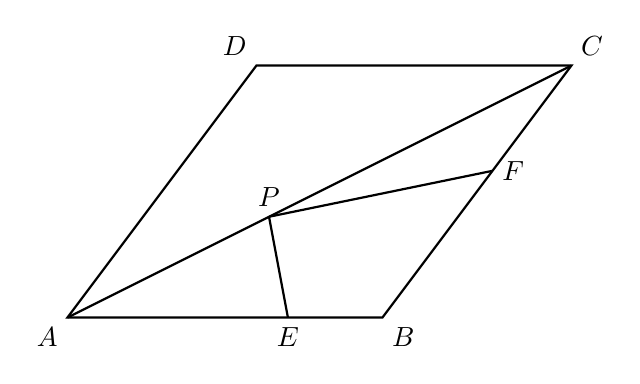
\begin{tikzpicture}[scale=0.8]
  \coordinate (A) at (0,0);
  \coordinate (B) at (5,0);
  \coordinate (C) at (8,4);
  \coordinate (D) at (3,4);
  \coordinate (E) at (3.5,0);
  \coordinate (P) at (3.2,1.6);
  \coordinate (F) at (6.75,2.33);

  \draw[thick] (A) -- (B) -- (C) -- (D) -- cycle;
  \draw[thick] (A) -- (C);
  \draw[thick] (P) -- (E);
  \draw[thick] (P) -- (F);

  \node[above left] at (D) {$D$};
  \node[above right] at (C) {$C$};
  \node[right] at (F) {$F$};
  \node[above] at (P) {$P$};
  \node[below left] at (A) {$A$};
  \node[below] at (E) {$E$};
  \node[below right] at (B) {$B$};
\end{tikzpicture}
\end{document}
